% Problem Statement
\chapter{Problem Statement} \label{ch:problem}

This thesis considers two control problems, which will be described in Sections \ref{sec:siso_problem} and \ref{sec:mimo_problem}, and addressed in Chapters \ref{ch:siso_shared_ctrl} and \ref{ch:mimo_shared_ctrl}, respectively. In the first problem, it is assumed that the plant has a single input and single output, and that the full state of the plant is measured directly. In this problem it is also assumed that the plant is an aircraft which has a pilot on-board. In the second problem, the plant is assumed to have multiple inputs and multiple outputs, while only the plant outputs are measured. In this second problem, the plant is assumed to be an unmanned aircraft with a remote human operator. This thesis posits that both of these problems may be addressed by designing shared control architectures which make use of collaboration between humans and adaptive control algorithms.

\section{Aircraft with On-Board Human Pilot and Full State Measurements} \label{sec:siso_problem}

We consider single-input single-output (SISO) \textit{n}th-order linear dynamical plant models of the form 
\begin{equation}
\dot x_p = A_p x_p + B_p u_p	, \qquad y_p = C_p x_p \label{eq:siso_plant}
\end{equation} 
\noindent where $x_p(t) \in \mathbb{R}^{n \times 1}$ is the state vector, $A_p \in \mathbb{R}^{n \times n}$ and $B_p \in \mathbb{R}^{n \times 1}$ are an uncertain matrix and an uncertain vector of dynamical properties, respectively, and $u_p(t)$ is a scalar input. $C_p \in \mathbb{R}^{1 \times n}$ is a known vector producing the scalar plant output, $y_p(t)$, which we would like to follow prescribed commands $r(t)$ by providing a control action $u(t)$. For this problem, we consider the case where the vector $x_p$, consisting of the output $y_p$ and its first $n-1$ time derivatives, is measured and available for use in feedback control, and the vector $B_p$ is given by $B_p = [0, \cdots \, 0, \, \beta]^T$. We note that plants of this form have a transfer function from plant input to output given in the Laplace frequency domain by
\begin{equation}
\frac{Y_p(s)}{U_p(s)} = \frac{\beta}{s^n + \alpha_{n-1} s^{n-1} + \cdots + \alpha_0}	
\end{equation}
where $\alpha_i$ and $\beta$ are arbitrary coefficients. Design of the control law $u(t)$ is carried out under nominal conditions with the assumption
\begin{equation}
	u_p(t) \equiv u(t). \label{eq:siso_plant_input_nom}
\end{equation}
Note that uncertainty in control effectiveness is captured by the uncertain matrix $B_p$. 

In addition to an autonomous controller which generates control input $u(t)$ in (\ref{eq:siso_plant_input_nom}), a human operator (pilot) is tasked with the high-level operation of the plant (\ref{eq:siso_plant}), including monitoring to ensure safe and anomaly-free operation. Operation is denoted \textit{human-on-the-loop} as opposed to \textit{human-in-the-loop}, as the pilot does not directly command actuator input. The pilot's perceptive capabilities (corresponding to the pathways in Figure \ref{fig:sheridan_adapted}) are assumed to include the sensing of $y_{D} \subseteq y$, $y_{H}$, and $r$, where $y_{D}$ is a subset of vehicle sensor measurements available to the pilot through cockpit displays, $y_{H}$ is the human pilot's sensing through visual and vestibular modalities, and $r$ is the prescribed command which the plant output should track. Note that in the single output case, $y_D \equiv y$.

%An adaptive autopilot based on model reference adaptive control (MRAC) is capable of addressing anomalies that can be represented as parametric uncertainties, but may perform poorly when an anomaly causes the order of the vehicle dynamics to change \cite{narendra2012stable, lavretsky2013robust}. A human pilot flying manually may detect such an anomaly and adapt to the anomalous dynamics, but the pilot's tracking performance may be noticeably poorer after a change in dynamics and pilot adaptation \cite{hess2015modeling, zaal2016manual}. 

We consider the introduction of two severe anomalies in the dynamics of the plant model (\ref{eq:siso_plant}), described in Sections \ref{subsec:siso_act_fault} and \ref{subsec:siso_delay}. The first consists of a change in the actuator dynamics, represented as a change in the actuator model from a gain to a first-order lag. The second anomaly is a latency introduced in the feedback of state information to the control algorithms. 

%The remote human supervisor has information on plant sensor measurements, state estimate, tracking performance, and health (via visual, haptic, and/or auditory interfaces). \textit{Human-in-the-loop} operation is possible via remote controls, allowing the operator to actuate the plant by manually providing $u(t)$ in (\ref{eq:first_order_act}) and (\ref{eq:second_order_act}). The sensing and actuation by the remote human supervisor include time delays $\tau_s, \tau_a > 0$, respectively.

The problem we investigate in Chapter \ref{ch:siso_shared_ctrl} is whether the design of $u(t)$ can be carried out using a shared decision-making and control architecture which leverages the merits of 
\begin{enumerate}[label=(\alph*)]
	\item autonomous control methodologies
	\item an on-board human pilot
\end{enumerate}
to successfully mitigate two types of anomalous dynamics to be described presently and restore tracking performance in the presence of uncertainty. We refer to this class of anomaly response as a shared control response. The following two subsections describe two specific anomalies which will be addressed using this shared controller in Chapter \ref{ch:siso_shared_ctrl}.

\subsection{Actuator Fault} \label{subsec:siso_act_fault}
An anomaly is introduced which changes the actuator dynamics from a direct input (\ref{eq:siso_plant_input_nom}) to a first-order lag
\begin{equation}
	T_L\dot{u}(t) + u(t) = u_p(t) \label{eqn:actuator_dynamics_symbolic}
\end{equation} 
\noindent so that the dynamics of plant augmented with actuator dynamics change suddenly from order $n$ to order $n+1$. We can define an augmented plant 
\begin{equation}
	\dot{x}_p' = A_p' x_p' + B_p' u	\label{eqn:plant_3_compact}
\end{equation}
where $u(t)$ is defined in (\ref{eqn:actuator_dynamics_symbolic}), and $x_p'(t)$ consists of the output $y_p(t)$ and its first $n$ time derivatives. The matrix $A_p'$ and vector $B_p'$ are then given by
\begin{equation}
	A_p' = \begin{bmatrix}
		\begin{matrix}0 \\ \vdots \end{matrix} & \Bigg[ \quad I_n \quad ~ \Bigg] \\ \alpha_0' & \begin{matrix}\cdots & \alpha_{n+1}' \end{matrix}
	\end{bmatrix}, \quad B_p' = \begin{bmatrix}
		0 \\ \vdots \\ \beta'
	\end{bmatrix}
	\label{eqn:plant_3_symbolic}
\end{equation}
%\begin{equation}
%	\underbrace{\begin{bmatrix}
%		\dot{\phi} \\ \dot{p} \\ \ddot{p}
%	\end{bmatrix}}_{\dot{x}_p'} = \underbrace{\begin{bmatrix}
%		0 & 1 & 0\\ 0 & 0 & 1 \\ 0 & \frac{L_p}{T_L} & L_p - \frac{1}{T_L}
%	\end{bmatrix}}_{A_p'} \underbrace{\begin{bmatrix}
%		\phi \\ p \\ \dot{p}
%	\end{bmatrix}}_{x_p'} + \underbrace{\begin{bmatrix}
%		0 \\ 0 \\ \frac{L_{\delta_a}}{T_l}
%	\end{bmatrix}}_{B_p'} u
%	\label{eqn:plant_3_symbolic}
%\end{equation}
where $I_n$ is the identity matrix of dimension $n$ and $\alpha_i', \, \beta'$ are uncertain coefficients. If the change in the order of the plant is not known to the adaptive controller, it may no longer be possible for it to stabilize the plant following such a change. The question then is if a shared decision-making architecture, with suitable action from the human pilot leading to feedback on the augmented state vector $x_p'$, can result in the recovery of closed-loop performance with anomalous actuator model (\ref{eqn:actuator_dynamics_symbolic}) and parametric uncertainties in the plant (\ref{eqn:plant_3_compact}).

\subsection{Time-Delayed Sensor Measurements} \label{subsec:siso_delay}
We consider the introduction of an anomaly which leads to latency in the measurement of plant state information. We model this anomaly as the addition of a time delay $\tau$ of the state measurements before the computation of the control input, causing a discrepancy between the current plant state $x_p(t)$ and the state as sensed by the controller, denoted $x_\sigma(t)$, given by
\begin{equation}
	x_\sigma(t) = x_p(t - \tau). \label{eqn:delay_diffeq}
\end{equation}

We note that the effect of the time delay $\tau$ may be approximated as a first-order filter, given in the Laplace frequency domain as
\begin{equation}
	e^{-\tau s} \approx \frac{1}{1 + \tau s}.
\end{equation}
In the time domain, this approximation corresponds to the differential equation
\begin{equation}
	\tau \dot{x}_{\sigma}(t) + x_{\sigma}(t) \approx x_p(t)	\label{eqn:delay_approx_diffeq}
\end{equation}

We note that this effectively increases the order of the plant from $n$ to $n+1$ when we consider the output to be the delayed signal. In this case, using the time delay approximation of (\ref{eqn:delay_approx_diffeq}), the augmented plant model is given by
\begin{equation}
	\dot{x}_\sigma' = A_p' x_\sigma' + B_p' u \label{eqn:plant_3_tau}
\end{equation}
with $A_p'$ and $B_p'$ defined in (\ref{eqn:plant_3_symbolic}). Due to this similarity, we investigate the applicability of a shared control solution to the problem of Section \ref{subsec:siso_act_fault} to the problem of a time-delayed state measurement. The shared control architecture which we propose to address these two problems is presented in Chapter \ref{ch:siso_shared_ctrl}.

%\begin{equation}
%	\underbrace{\begin{bmatrix}
%		\dot{\phi} \\ \dot{p} \\ \ddot{p}
%	\end{bmatrix}}_{\dot{x}_\sigma'} = \underbrace{\begin{bmatrix}
%		0 & 1 & 0\\ 0 & 0 & 1 \\ 0 & \frac{L_p}{\tau} & L_p - \frac{1}{\tau}
%	\end{bmatrix}}_{A_\sigma'} \underbrace{\begin{bmatrix}
%		\phi \\ p \\ \dot{p}
%	\end{bmatrix}}_{x_\sigma'} + \underbrace{\begin{bmatrix}
%		0 \\ 0 \\ \frac{L_{\delta_a}}{\tau}
%	\end{bmatrix}}_{B_\sigma'} u
%	\label{eqn:plant_3_tau}
%\end{equation}

\section{Aircraft with Remote Human Pilot and Output Measurements}  \label{sec:mimo_problem}
Here we consider the problem of controlling linear multi-input multi-output (MIMO) plant models of the form
\begin{equation}
\begin{gathered}
\dot x_p = (A_p + B_p \Theta_p^T) x_p + B_p \Lambda_p u_p \\
y_p = C_p x_p, \qquad z_p = C_{pz} x_p \label{eq:plant_dynamics}
\end{gathered}
\end{equation}
where $x_p$ is the plant state, $u_p$ is the plant input, $y_p$ is measured output, and $z_p$ is regulated output. Uncertain dynamics lead to the introduction of unknown $\Theta_p$ and $\Lambda_p$ in the plant model. It is assumed that the matrix $CB$ has full rank, and thus the plant has uniform relative degree one (see \cite{qu2016adaptive}). In addition to the dynamics (\ref{eq:plant_dynamics}), the plant's actuators have the first-order dynamics
\begin{equation}
	\dot{u}_p + (D_1 + \Theta_1^T) u_p = D_1 u \label{eq:first_order_act}
\end{equation}
where $D_1$ is a diagonal matrix representing nominal actuator parameters and $\Theta_1$ models uncertainty in the actuator dynamics. The problem is to choose $u(t)$ such that $z_p(t)$ tracks an external command $z_{cmd}(t)$ as closely as possible.
%Model reference adaptive control (MRAC) with output feedback and closed-loop reference models, such as the method of \cite{qu2016adaptive}, can achieve asymptotic tracking and guarantee stability for this control problem. 

\subsection{Actuator Fault} \label{subsec:mimo_act_fault}
Consider the occurrence of an anomaly which causes an abrupt change in actuator dynamics from (\ref{eq:first_order_act}) to the second-order model
\begin{equation}
	\ddot{u}_p + (D_2 + \Theta_2^T) \dot{u}_p + (D_1 + \Theta_1^T) u_p = D_1 u \label{eq:second_order_act}
\end{equation}
where in addition to $\Theta_1$, $\Theta_2$ is an unknown parameter as well. This change in dynamics means that the the structure of the model used for control design is no longer accurate, and the autonomous controller may lose stability and command tracking ability. In particular, the challenge from the anomaly is the increase in relative degree between $u$ and $y_p$ from two to three.

In addition to an autonomous controller which generates control input $u(t)$ in (\ref{eq:first_order_act}) and (\ref{eq:second_order_act}), a human supervisor is tasked with the high-level operation of the plant (\ref{eq:plant_dynamics}), including mission and task planning (commanding its mode of operation) and monitoring to ensure safe and anomaly-free operation. In this chapter, we consider \textit{remote} human operators who cannot sense the vehicle state and dynamics directly through vestibular pathways. The human supervisor may be responsible for the supervision of multiple plant instances, as illustrated in Figure \ref{fig:uav_supervisor} for a highly flexible UAV platform. Operation is denoted \textit{human-on-the-loop} in the same manner as the on-board human pilot considered in the problem of Section \ref{sec:siso_problem}. 

\begin{figure}[htbp]
	\centering
	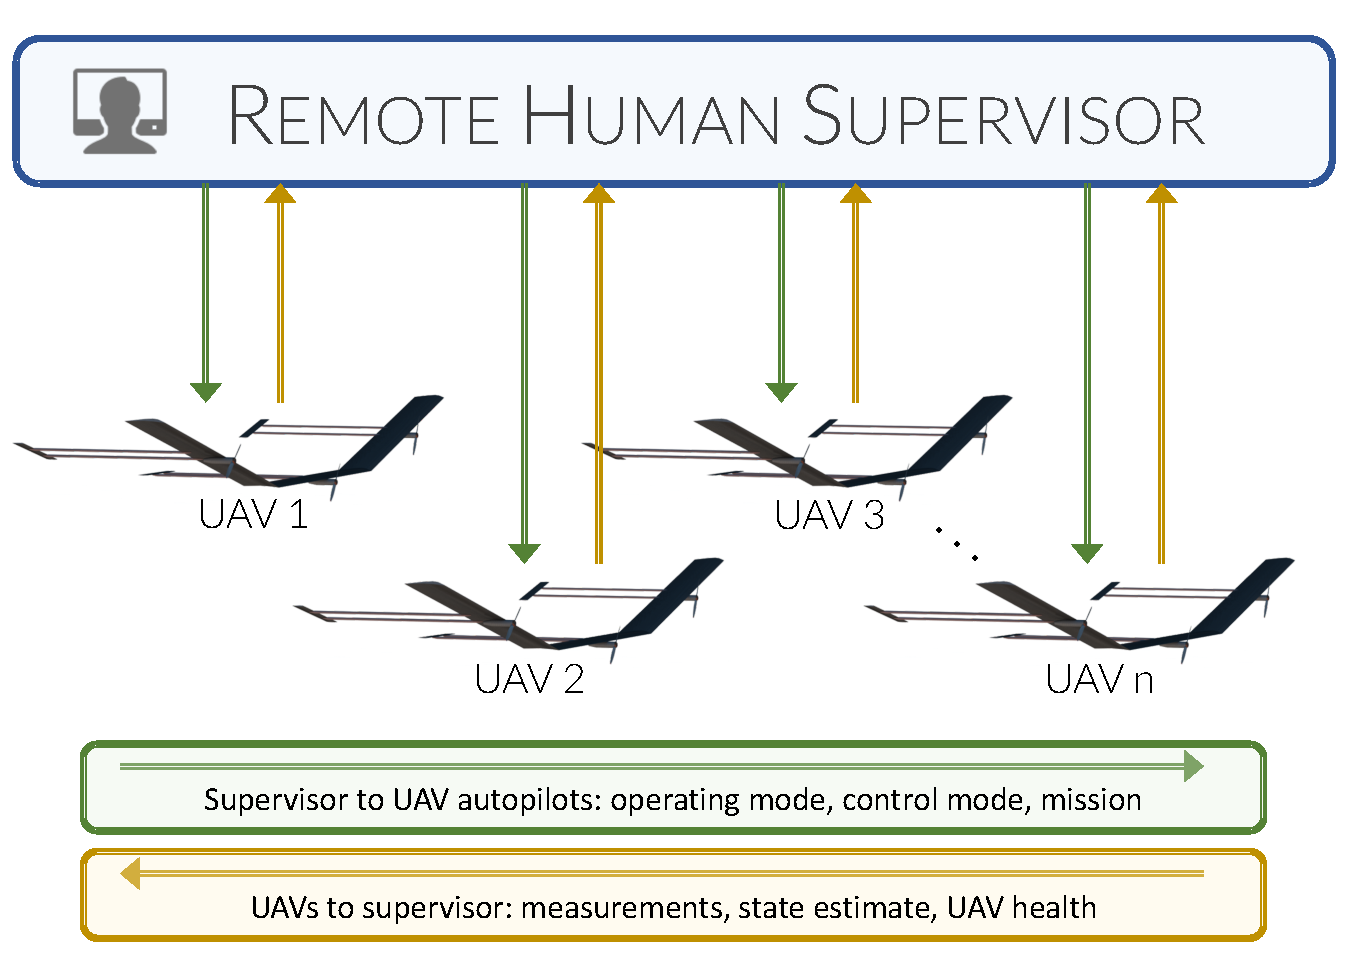
\includegraphics[width=0.95\columnwidth]{uav_supervisor.pdf}
	\caption{Supervisory operation of a fleet of high altitude, long endurance UAVs by remote human operator}
	\label{fig:uav_supervisor}
\end{figure}

It is assumed that the human supervisor has access to information on plant sensor measurements, state estimate, tracking performance, and health (via visual, haptic, and/or auditory interfaces), and is able to perceive changes in plant dynamics, such as an increased lag or decreased control effectiveness, via these interfaces.  \textit{Human-in-the-loop} operation is possible via remote controls, allowing the operator to actuate the plant by manually providing $u(t)$ in (\ref{eq:first_order_act}) and (\ref{eq:second_order_act}). The sensing and actuation by the remote human supervisor include time delays $\tau_s, \tau_a > 0$, respectively.

The problem we investigate in Chapter \ref{ch:mimo_shared_ctrl} is whether the design of $u(t)$ can be carried out using a shared decision-making and control architecture which combines
\begin{enumerate}[label=(\alph*)]
	\item autonomous control methodologies
	\item a remote human supervisor
\end{enumerate}
so as to lead to a successful mitigation of an abrupt anomaly causing a change from (\ref{eq:first_order_act}) to (\ref{eq:second_order_act}) and restore tracking performance in the presence of uncertainty. This problem is a natural extension of the problem introduced in Section \ref{sec:siso_problem}, where the solution must additionally accommodate
\begin{enumerate}[label=(\roman*)]
	\item multi-input, multi-output plants;
	\item unmeasured state variables;
	\item remote human operators.
\end{enumerate}
The shared control solution proposed in Chapter \ref{ch:mimo_shared_ctrl} of this thesis will thus build on the shared controller described in Chapter \ref{ch:siso_shared_ctrl}.
  
%  We refer to this class of anomaly response as a shared control response. This work builds on anomaly response frameworks using adaptive autopilots and on-board human pilots reported in \cite{farjadian2017bumpless} and \cite{thomsen2018shared}.
